\documentclass[11pt,a4paper]{article}
\usepackage[margin=2.2cm]{geometry}
\usepackage{graphicx,booktabs,xcolor,array,float}
\usepackage[hidelinks]{hyperref}
\usepackage{fancyhdr}
\pagestyle{fancy}\fancyhf{}
\lhead{34870 Loudspeaker project -- lab results 12 Nov 2026}\rhead{Group 10, System D}\cfoot{\thepage}
\setlength{\parskip}{4pt}\setlength{\parindent}{0pt}
\newcommand{\good}{\textcolor{green!50!black}{\textbf{good}}}
\newcommand{\fix}{\textcolor{orange!85!black}{\textbf{to fix}}}
\newcommand{\open}{\textcolor{blue!60!black}{\textbf{open}}}
\begin{document}

{\LARGE\bfseries Lab day 12 November: results}\\[2pt]
{\large 34870 Electroacoustics, loudspeaker project, Group 10 (System D), anechoic chamber}\\[2pt]
{\small Data: \texttt{lab-day/data/2026-11-12/} (labgui files, unchanged from the lab PC). Figures and numbers:
\texttt{lab-day/analysis/results\_1112.m}. Short version: \texttt{RESULTS.md} in this folder.}

\section*{In one paragraph}
The crossover design works. With the MiniDSP mistake removed, System D is flat to
\textbf{5.5\,dB peak-to-peak (1.23\,dB rms) from 150\,Hz to 15\,kHz} on axis. On 10 November it was
7.1\,dB, and the prediction for the new tweeter resistor was 5.3\,dB. The big dip we saw at 300--450\,Hz
was not the speaker: the LR4 high-pass on MiniDSP Output~2 had been entered \textbf{twice}, which turned
the midrange about 140\textdegree\ against the woofer so the two partly cancelled. Changing the tweeter
L-pad resistor \textbf{Rp from 3.3\,$\Omega$ to 8.2\,$\Omega$} raised the tweeter by 2.9\,dB, as predicted
from the 10-Nov data. The speaker sat exactly where it did in Lab E. The one thing missing is a
measurement with the corrected MiniDSP: the 5.5\,dB is computed from run S\_3, not measured.

\begin{center}\small
\begin{tabular}{@{}>{\raggedright}p{6.0cm}>{\raggedright}p{6.8cm}l@{}}\toprule
Quantity & Result & Verdict\\\midrule
Placement vs Lab E (run P) & same shape within 0.2--0.7\,dB rms, all units $+2.2$\,dB & \good\\
Woofer channel vs 10-Nov (S\_3) & within 0.2\,dB, 150\,Hz--1\,kHz & \good\\
MiniDSP Output 2 & LR4 high-pass applied twice (misfit 0.6\,dB rms) & \fix\ (fixed in the lab)\\
Woofer -- mid phase at 325\,Hz & $-141$\textdegree\ as measured, $+10$\textdegree\ with the extra filter removed & \good\ once fixed\\
Rp 3.3 $\rightarrow$ 8.2\,$\Omega$ & $+2.9$\,dB at 5--15\,kHz, prediction within 0.3\,dB to 10\,kHz & \good\\
On-axis spread 150\,Hz--15\,kHz & 5.5\,dB / 1.23\,dB rms (computed) & \good\\
System with the corrected MiniDSP & not measured & \open\\\bottomrule
\end{tabular}
\end{center}

\section{What was measured}
Placement as in Lab E: UMIK on axis, 1.15\,m high, 2.44\,m from the baffle (2.26\,m for S\_4 and S\_5).
The units were selected on the chamber's switchboard. One run holds three states recorded back to back,
so the states inside one run are phase-coherent; separate runs are not (the UMIK has its own USB clock).

\begin{center}\small
\begin{tabular}{@{}>{\raggedright}p{4.6cm}>{\raggedright\arraybackslash}p{10.6cm}@{}}\toprule
Part of the chain & Setting on 12 Nov\\\midrule
MiniDSP Output 1 (woofer) & LR4 low-pass 325\,Hz (\texttt{data/dsp/MiniDSP\_woofer\_out1.txt}), gain $-5.8$\,dB; raised by about 4.5\,dB before S\_5 (value not logged)\\
MiniDSP Output 2 (mid + tweeter) & LR4 high-pass 325\,Hz (\texttt{MiniDSP\_midtw\_out2.txt}), gain 0\,dB; \textbf{entered twice by mistake} in every S run\\
MiniDSP, other & no invert, no delay, PEQ / Comp / FIR bypassed, 96\,kHz\\
Amplifier & Dynavox CS-PA1 MKII, volume about 11 o'clock, bass and treble centred, input 2\\
Passive board, midrange & L\_mid 0.82\,mH in series, C\_mid 6.8\,\textmu F across the driver\\
Passive board, tweeter & C\_tw 5.6\,\textmu F in series, L\_tw 0.22\,mH to ground, Rs 4.7\,$\Omega$, \textbf{Rp 8.2\,$\Omega$} (3.3\,$\Omega$ in S\_4)\\
Vent & 160\,mm for P and S; 200\,mm and open from S\_2 on\\\bottomrule
\end{tabular}
\end{center}

\begin{center}\small
\begin{tabular}{@{}lll>{\raggedright\arraybackslash}p{7.4cm}@{}}\toprule
Time & Run & What changed & Used?\\\midrule
13:19 & \textbf{P} & MiniDSP bypassed, units driven directly & \textbf{yes}: placement check\\
13:37 & S & full system, vent 160\,mm & no: amplifier channels swapped (``woofer only'' played the high-passed signal)\\
13:51 & S\_2 & vent 200\,mm and open, cables reseated & no: same channel swap\\
13:56 & \textbf{S\_3} & channels correct, Rp 8.2\,$\Omega$ & \textbf{yes}: main result\\
14:03 & \textbf{S\_4} & Rp back to 3.3\,$\Omega$, mic 2.26\,m & \textbf{yes}: reference for the Rp comparison\\
14:11 & S\_5 & Out 1 gain raised about 4.5\,dB & no: balance off by $+5.6$\,dB; a gain change cannot fix a phase problem\\\bottomrule
\end{tabular}
\end{center}
Two corrections to the handwritten notes: the swap in S and S\_2 was the amplifier channels, not the
GUI's columns (S\_3's own note says so), and in run P the units were driven directly, not through the board.

\section{Placement is the same as in Lab E}
\begin{figure}[H]\centering
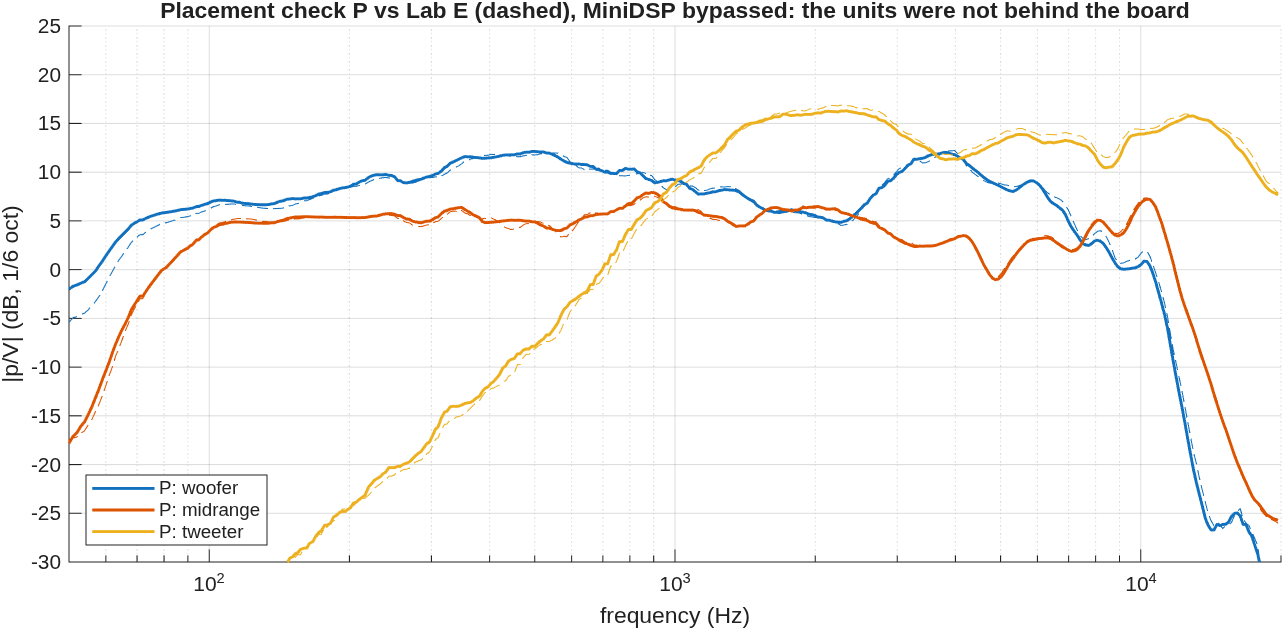
\includegraphics[width=\linewidth]{fig_placement.png}
\caption{Run P (solid) against the bare Lab E units (dashed), MiniDSP bypassed. Shape error after the level
offset: woofer 0.6, midrange 0.2, tweeter 0.7\,dB rms. All three are $+2.2$\,dB, which is amplifier volume.}
\label{fig:place}
\end{figure}
Figure~\ref{fig:place}: every unit lands on its Lab E curve. The Lab E model is therefore a fair reference
for this placement, and run P does not need repeating.

\section{The 300--450\,Hz dip: a doubled MiniDSP high-pass}
\begin{figure}[H]\centering
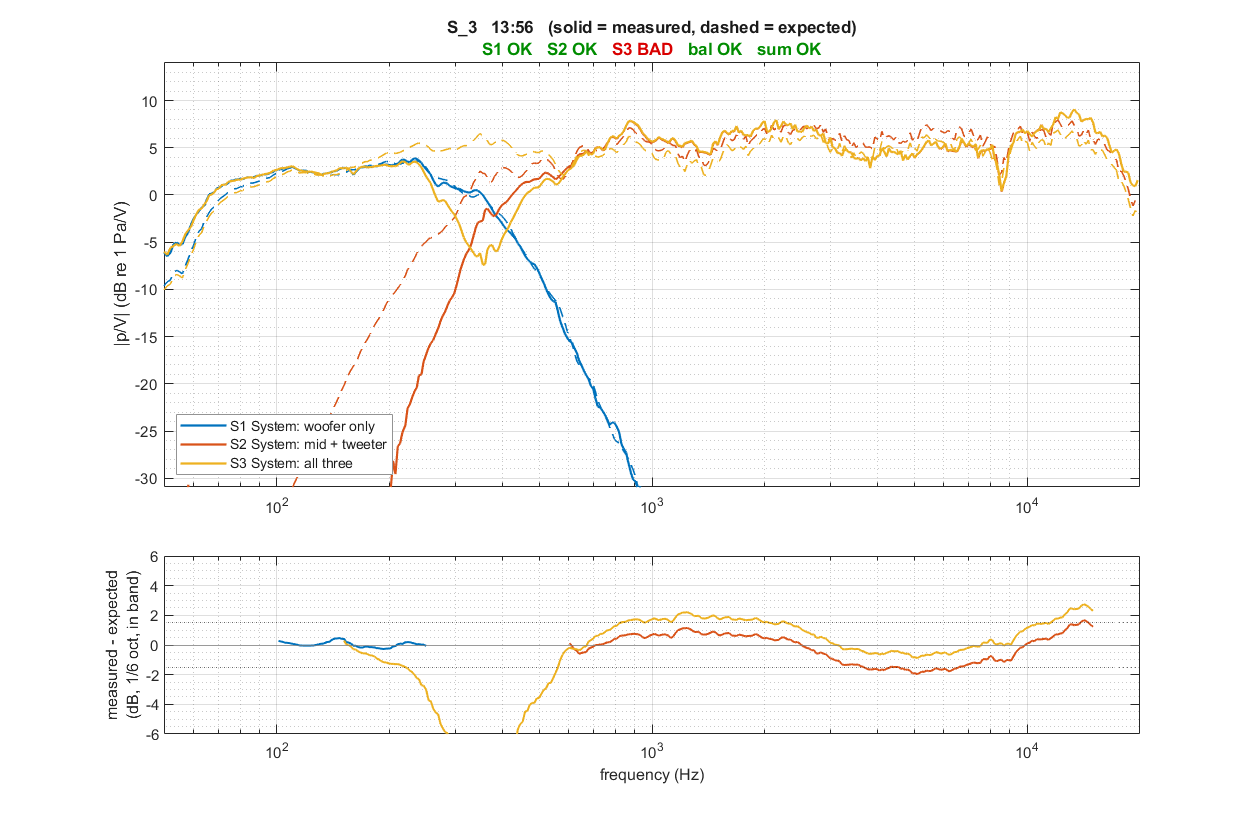
\includegraphics[width=\linewidth]{fig_S3_dashboard.png}
\caption{Run S\_3 as the lab GUI showed it (solid = measured, dashed = expected from the design).
The woofer (blue) sits on its expected curve; the mid + tweeter channel (red) falls far too early below
600\,Hz, and the sum (yellow) dips to about $-7$\,dB at 350--400\,Hz.}
\label{fig:dash}
\end{figure}

\begin{figure}[H]\centering
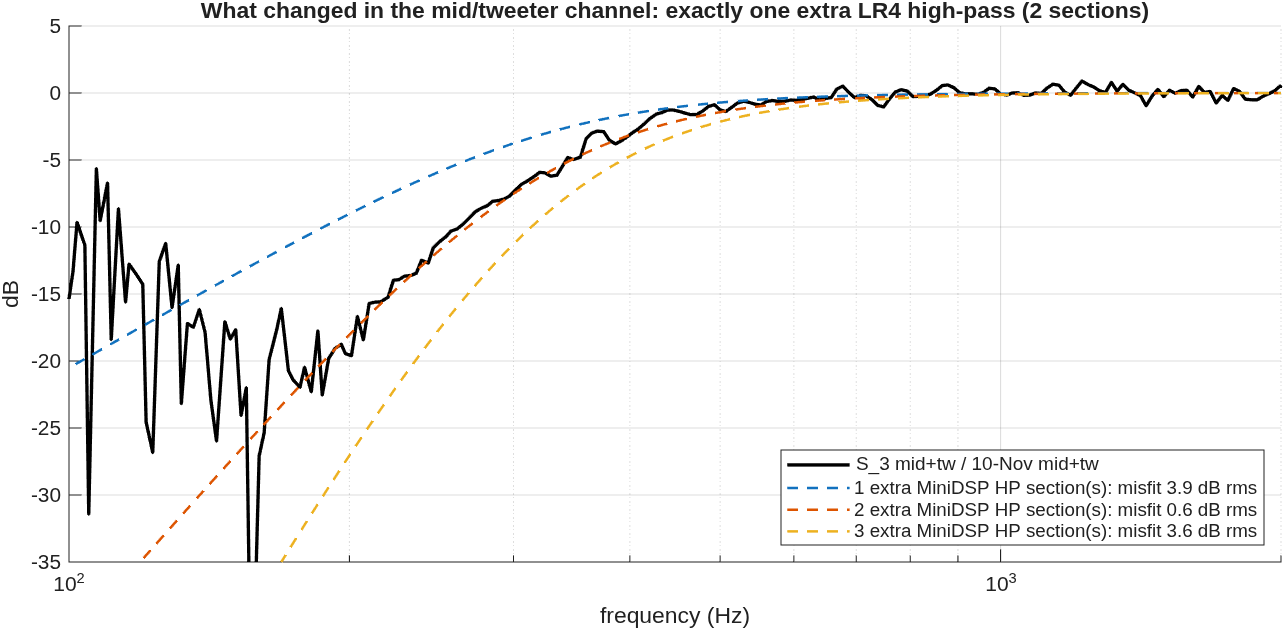
\includegraphics[width=\linewidth]{fig_double_filter.png}
\caption{The mid + tweeter channel of S\_3 divided by the same channel on 10 Nov, against 1, 2 and 3 extra
MiniDSP high-pass biquad sections. Two sections (one LR4) fit with 0.6\,dB rms; one or three misfit by 3.9 and 3.6\,dB.
Below 200\,Hz the ratio is noise.}
\label{fig:double}
\end{figure}

Figure~\ref{fig:dash} shows the problem the way we saw it in the lab: the woofer is fine, the mid + tweeter
channel is not. Dividing that channel by its 10-Nov version (Figure~\ref{fig:double}) leaves exactly one
extra LR4 high-pass at 325\,Hz, i.e. the Output~2 filter applied twice. The sum check confirms it is
cancellation and not a broken driver: $|$S1 + S2$|$ equals the measured S3 within 0.1\,dB.

\begin{figure}[H]\centering
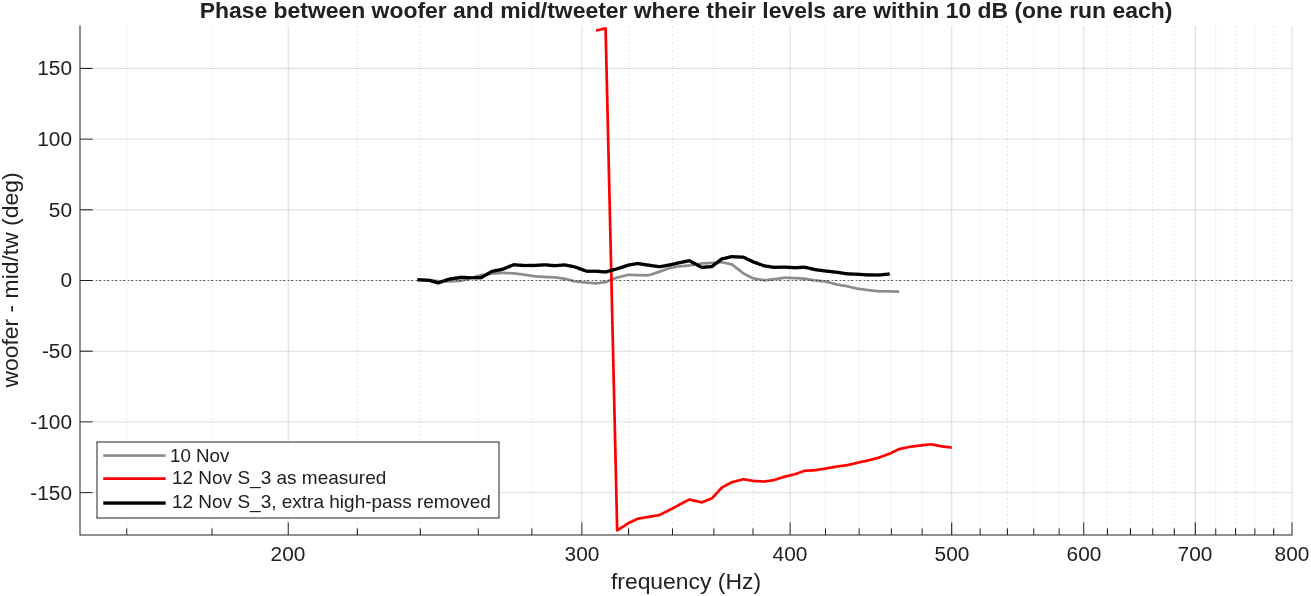
\includegraphics[width=\linewidth]{fig_phase.png}
\caption{Phase between the woofer and the mid/tweeter channel where their levels are within 10\,dB, each from
one run. 10 Nov: about 0\textdegree. S\_3 as measured: $-141$\textdegree\ at 325\,Hz (the jump at 310\,Hz is only the
$\pm180$\textdegree\ wrap). S\_3 with the extra filter removed: about $+10$\textdegree.}
\label{fig:phase}
\end{figure}

Why a doubled filter makes a hole instead of just a weaker midrange: an LR4 high-pass turns the phase by
180\textdegree\ at its corner frequency. The second copy turns the midrange another 140--180\textdegree\ around 325\,Hz,
so it arrives nearly in anti-phase with the woofer (Figure~\ref{fig:phase}) and the two cancel, by up to
11\,dB at 400\,Hz. That is also why raising the woofer gain in S\_5 made the balance worse instead of
better. The filter was corrected in the MiniDSP after S\_5; no run was taken afterwards.

\section{The tweeter fix: Rp 3.3 $\rightarrow$ 8.2\,$\Omega$}
\begin{figure}[H]\centering
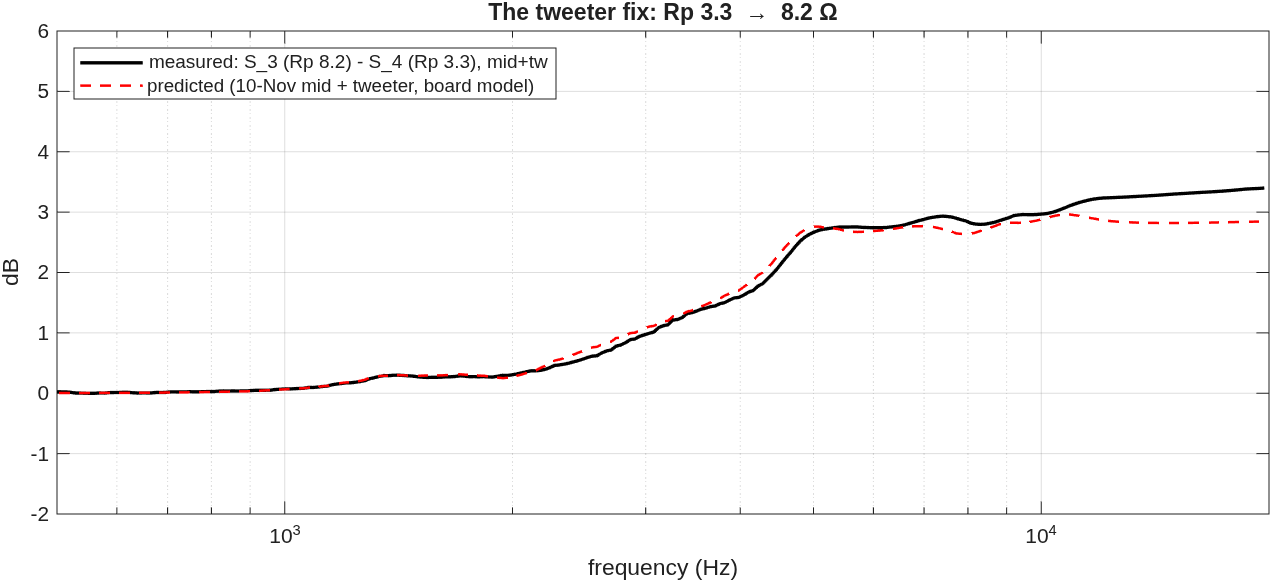
\includegraphics[width=\linewidth]{fig_rp.png}
\caption{S\_3 (Rp 8.2) minus S\_4 (Rp 3.3), mid + tweeter channel, against the prediction made from the
10-Nov units and the board model (\texttt{analysis/pad\_predict.m}).}
\label{fig:rp}
\end{figure}
S\_3 and S\_4 share the same (doubled) MiniDSP setting, so their difference isolates the resistor
(Figure~\ref{fig:rp}). The tweeter band rises by 2.9\,dB (5--15\,kHz) and 1--3\,kHz by only 0.3\,dB.
The prediction holds within about 0.3\,dB up to 10\,kHz; above that the measured lift is slightly larger
($+3.3$\,dB at 15\,kHz). The microphone moved from 2.44 to 2.26\,m between the runs, which explains a few tenths.

\section{The system with both fixes}
\begin{figure}[H]\centering
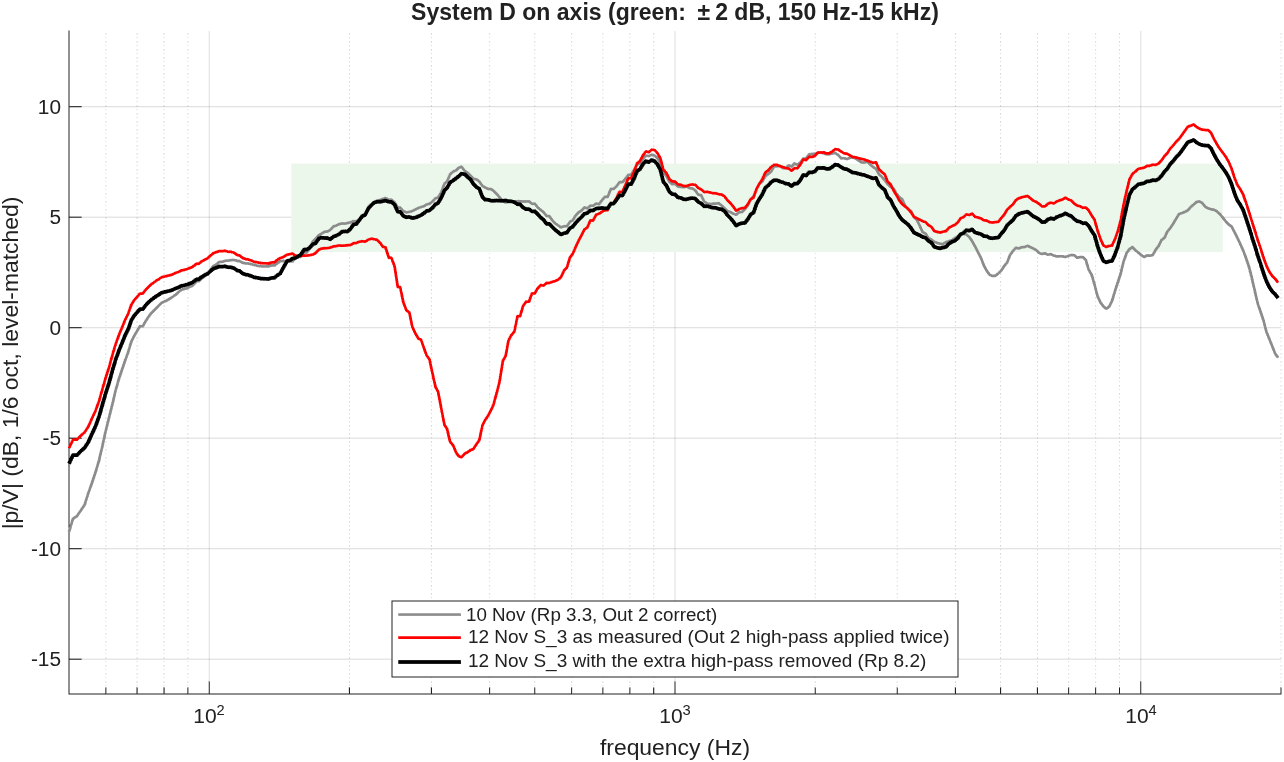
\includegraphics[width=\linewidth]{fig_system.png}
\caption{System D on axis, 1/6 octave, level-matched. Grey: 10 Nov (Rp 3.3, correct MiniDSP). Red: S\_3 as
measured. Black: S\_3 with the extra high-pass removed by calculation (Rp 8.2). Green band: $\pm2$\,dB,
150\,Hz--15\,kHz.}
\label{fig:sys}
\end{figure}

Because S\_3's three states are phase-coherent, the extra high-pass can be divided out of the mid + tweeter
state and the two channels summed again. The result (black in Figure~\ref{fig:sys}) is what the speaker
should sound like now:

\begin{center}\small
\begin{tabular}{@{}lcc@{}}\toprule
On-axis response, 150\,Hz--15\,kHz, 1/6 octave & Peak-to-peak & rms\\\midrule
Prediction for Rp 8.2\,$\Omega$ (from 10-Nov) & 5.3\,dB & 1.20\,dB\\
\textbf{12 Nov S\_3, extra filter removed, Rp 8.2\,$\Omega$} & \textbf{5.5\,dB} & \textbf{1.23\,dB}\\
10 Nov measured, Rp 3.3\,$\Omega$ & 7.1\,dB & 1.60\,dB\\
12 Nov S\_4, extra filter removed, Rp 3.3\,$\Omega$ & 7.4\,dB & 1.72\,dB\\
12 Nov S\_3 as measured (doubled filter) & 15.1\,dB & 3.39\,dB\\\bottomrule
\end{tabular}
\end{center}

Three features remain, and listeners may notice them:
\begin{itemize}\itemsep0pt
\item a broad plateau about 1.5\,dB high at 1.5--3\,kHz (the midrange's own response; needs a different mid filter),
\item a narrow dip at 8.3\,kHz (already in the tweeter's Lab E response; the crossover cannot remove it),
\item a peak about 1\,dB above the $\pm2$\,dB band at 11--14\,kHz, now that the tweeter is louder.
\end{itemize}
Below about 120\,Hz S\_3 sits above 10-Nov because the vent was open from S\_2 on; the chamber is not valid
there anyway (the low end is the near-field measurement from Lab D and 10-Nov).

\section{The hardware as used}
\begin{figure}[H]\centering
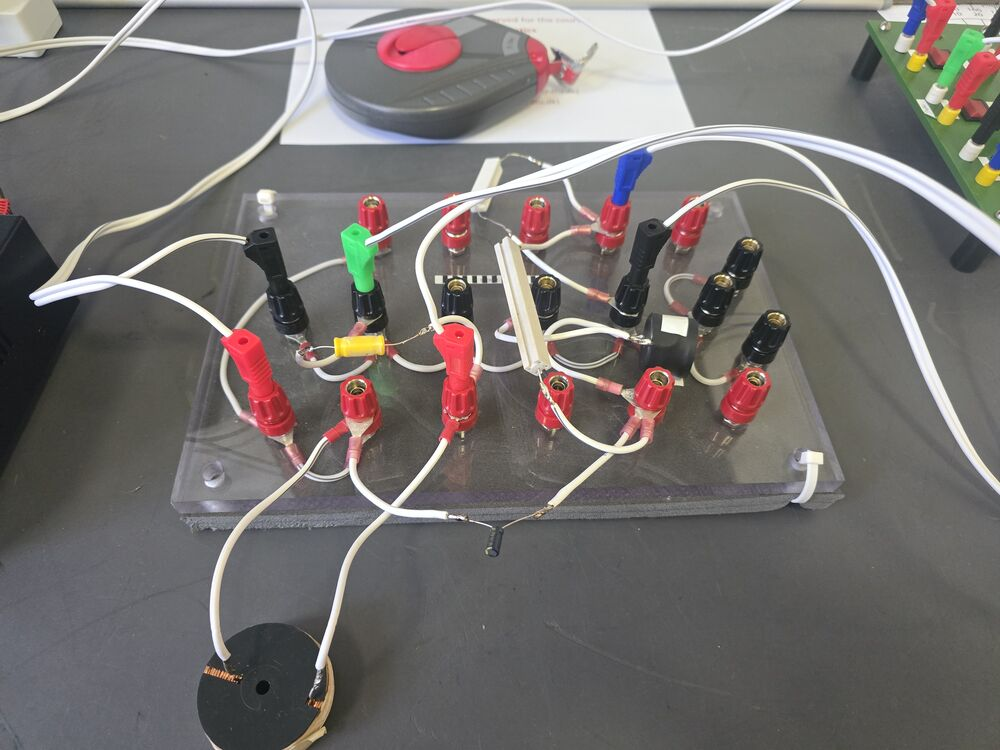
\includegraphics[width=0.62\linewidth]{photos/board.jpg}
\caption{The passive crossover board as built on 12 Nov (midrange LP2, tweeter HP2 + L-pad).}
\end{figure}
\begin{figure}[H]\centering
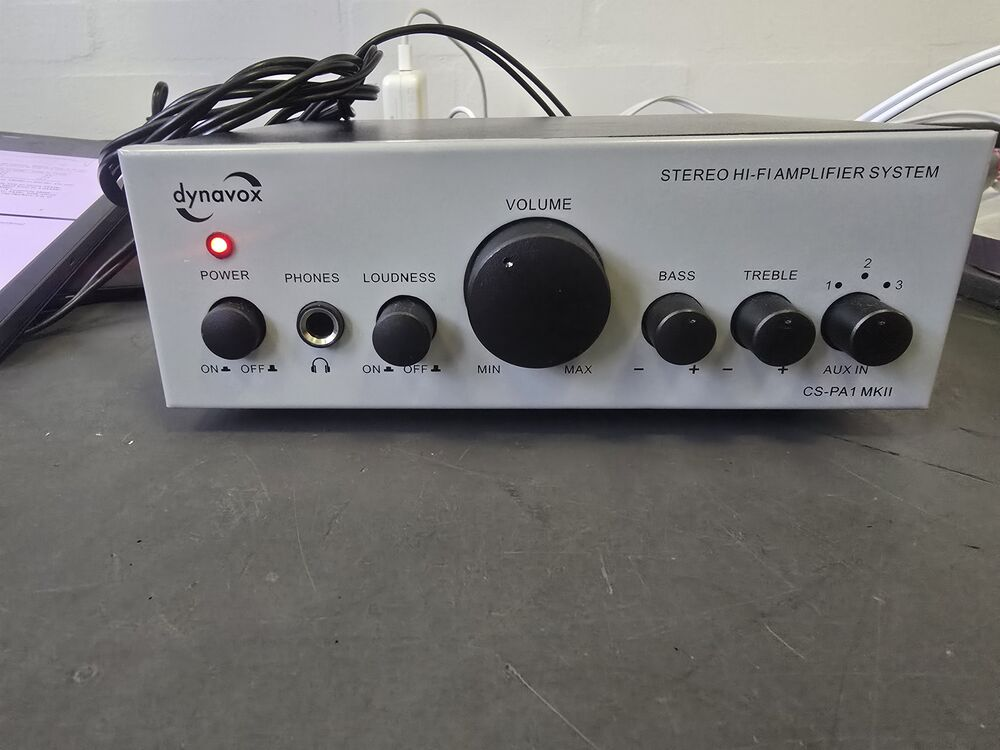
\includegraphics[height=5.2cm]{photos/amplifier.jpg}\hfill
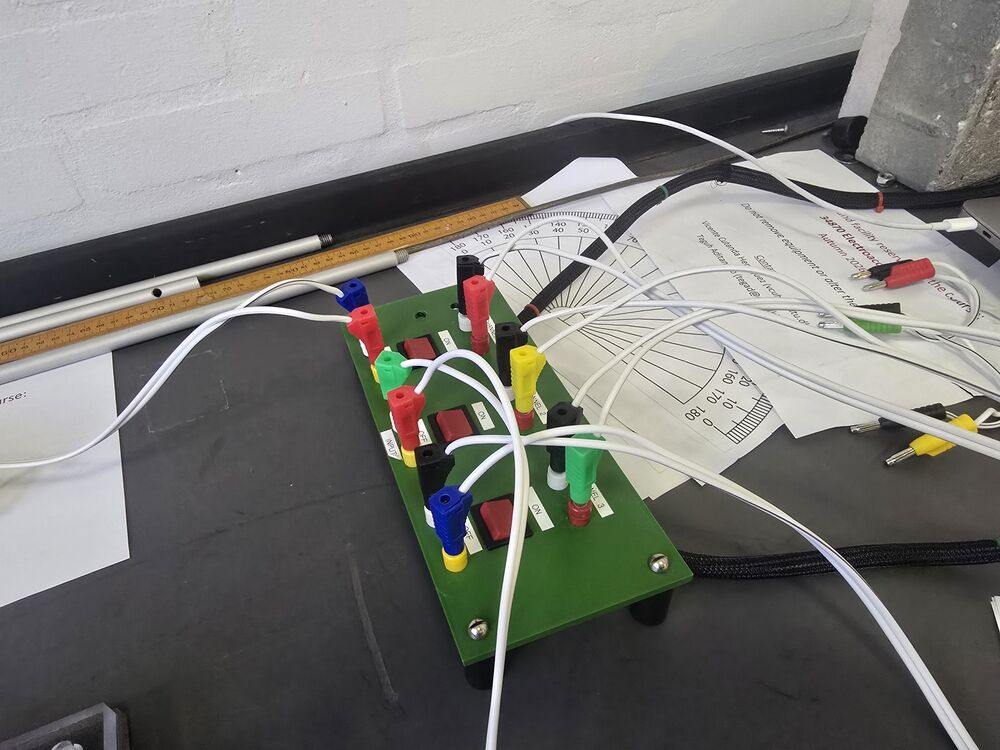
\includegraphics[height=5.2cm]{photos/switchboard.jpg}
\caption{Left: the chamber amplifier (volume about 11 o'clock, bass and treble centred, input 2).
Right: the switchboard that selects woofer, midrange and tweeter.}
\end{figure}

\section{What this means for the listening test}
\begin{enumerate}\itemsep2pt
\item \textbf{MiniDSP Output 2 must hold exactly the two biquads} from \texttt{MiniDSP\_midtw\_out2.txt}, nothing
else. The IEC room has its own MiniDSP card, so the filters are entered again there. Check with a 325\,Hz sine:
Output 2 is 6\,dB below its level at 1\,kHz; 12\,dB below means the filter is doubled again.
\item \textbf{Out 1 $=-5.8$\,dB, Out 2 $=0$\,dB, Rp $=8.2\,\Omega$.} The room's amplifier is not the chamber's, so
the woofer balance may be off by about a dB; the blind bass comparison in the listening test checks it by ear.
\item One vent open at 160\,mm, the other plugged (the design tuning, $f_B \approx 24.6$\,Hz).
\item If time allows, one \texttt{S} run in the chamber with the corrected MiniDSP confirms the 5.5\,dB.
\end{enumerate}

\end{document}
